%% History:
% Pavel Tvrdik (26.12.2004)
%  + initial version for PhD Report
%
% Daniel Sykora (27.01.2005)
%
% Michal Valenta (3.12.2008)
% rada zmen ve formatovani (diky M. Duškovi, J. Holubovi a J. Žďárkovi)
% sjednoceni zdrojoveho kodu pro anglickou, ceskou, bakalarskou a diplomovou praci

% One-page layout: (proof-)reading on display
%%%% \documentclass[11pt,oneside,a4paper]{book}
% Two-page layout: final printing
\documentclass[11pt,twoside,a4paper]{book}   
%=-=-=-=-=-=-=-=-=-=-=-=--=%
% The user of this template may find useful to have an alternative to these 
% officially suggested packages:
\usepackage[czech, english]{babel}
\usepackage[T1]{fontenc} % pouzije EC fonty 
% pripadne pisete-li cesky, pak lze zkusit take:
% \usepackage[OT1]{fontenc} 
\usepackage[utf8]{inputenc}
%=-=-=-=-=-=-=-=-=-=-=-=--=%
% In case of problems with PDF fonts, one may try to uncomment this line:
%\usepackage{lmodern}
%=-=-=-=-=-=-=-=-=-=-=-=--=%
%=-=-=-=-=-=-=-=-=-=-=-=--=%
% Depending on your particular TeX distribution and version of conversion tools 
% (dvips/dvipdf/ps2pdf), some (advanced | desperate) users may prefer to use 
% different settings.
% Please uncomment the following style and use your CSLaTeX (cslatex/pdfcslatex) 
% to process your work. Note however, this file is in UTF-8 and a conversion to 
% your native encoding may be required. Some settings below depend on babel 
% macros and should also be modified. See \selectlanguage \iflanguage.
%\usepackage{czech}  %%%%%\usepackage[T1]{czech} %%%%[IL2] [T1] [OT1]
%=-=-=-=-=-=-=-=-=-=-=-=--=%

%%%%%%%%%%%%%%%%%%%%%%%%%%%%%%%%%%%%%%%
% Styles required in your work follow %
%%%%%%%%%%%%%%%%%%%%%%%%%%%%%%%%%%%%%%%
\usepackage{graphicx}
\usepackage{indentfirst} %1. odstavec jako v cestine.
\usepackage{k336_thesis_macros} % specialni makra pro formatovani DP a BP
 % muzete si vytvorit i sva vlastni v souboru k336_thesis_macros.sty
 % najdete  radu jednoduchych definic, ktere zde ani nejsou pouzity
 % napriklad: 
 % \newcommand{\bfig}{\begin{figure}\begin{center}}
 % \newcommand{\efig}{\end{center}\end{figure}}
 % umoznuje pouzit prikaz \bfig namisto \begin{figure}\begin{center} atd.


%%%%%%%%%%%%%%%%%%%%%%%%%%%%%%%%%%%%%
% Zvolte jednu z moznosti 
% Choose one of the following options
%%%%%%%%%%%%%%%%%%%%%%%%%%%%%%%%%%%%%
%\newcommand\TypeOfWork{Diplomová práce} \typeout{Diplomova prace}
% \newcommand\TypeOfWork{Master's Thesis}   \typeout{Master's Thesis} 
 \newcommand\TypeOfWork{Bakalářská práce}  \typeout{Bakalarska prace}
% \newcommand\TypeOfWork{Bachelor's Project}  \typeout{Bachelor's Project}


%%%%%%%%%%%%%%%%%%%%%%%%%%%%%%%%%%%%%
% Zvolte jednu z moznosti 
% Choose one of the following options
%%%%%%%%%%%%%%%%%%%%%%%%%%%%%%%%%%%%%
% nabidky jsou z: http://www.fel.cvut.cz/cz/education/bk/prehled.html

%\newcommand\StudProgram{Elektrotechnika a informatika, dobíhající, Bakalářský}
%\newcommand\StudProgram{Elektrotechnika a informatika, dobíhající, Magisterský}
% \newcommand\StudProgram{Elektrotechnika a informatika, strukturovaný, Bakalářský}
% \newcommand\StudProgram{Elektrotechnika a informatika, strukturovaný, Navazující magisterský}
 \newcommand\StudProgram{Softwarové technologie a management, Bakalářský}
% English study:
% \newcommand\StudProgram{Electrical Engineering and Information Technology}  % bachelor programe
% \newcommand\StudProgram{Electrical Engineering and Information Technology}  %master program


%%%%%%%%%%%%%%%%%%%%%%%%%%%%%%%%%%%%%
% Zvolte jednu z moznosti 
% Choose one of the following options
%%%%%%%%%%%%%%%%%%%%%%%%%%%%%%%%%%%%%
% nabidky jsou z: http://www.fel.cvut.cz/cz/education/bk/prehled.html

%\newcommand\StudBranch{Výpočetní technika}   % pro program EaI bak. (dobihajici i strukt.)
%\newcommand\StudBranch{Výpočetní technika}   % pro prgoram EaI mag. (dobihajici i strukt.)
\newcommand\StudBranch{Softwarové inženýrství}            %pro STM
%\newcommand\StudBranch{Web a multimedia}                  % pro STM
%\newcommand\StudBranch{Computer Engineering}              % bachelor programe
%\newcommand\StudBranch{Computer Science and Engineering}  % master programe


%%%%%%%%%%%%%%%%%%%%%%%%%%%%%%%%%%%%%%%%%%%%
% Vyplnte nazev prace, autora a vedouciho
% Set up Work Title, Author and Supervisor
%%%%%%%%%%%%%%%%%%%%%%%%%%%%%%%%%%%%%%%%%%%%

\newcommand\WorkTitle{Demonstrační aplikace pro podporu kurzu neuronových sítí}
\newcommand\FirstandFamilyName{Adam Činčura}
\newcommand\Supervisor{Ing. Zdeněk Buk}


% Pouzijete-li pdflatex, tak je prijemne, kdyz bude mit vase prace
% funkcni odkazy i v pdf formatu
\usepackage[
pdftitle={\WorkTitle},
pdfauthor={\FirstandFamilyName},
bookmarks=true,
colorlinks=true,
breaklinks=true,
urlcolor=red,
citecolor=blue,
linkcolor=blue,
unicode=true,
]
{hyperref}



% Extension posted by Petr Dlouhy in order for better sources reference (\cite{} command) especially in Czech.
% April 2010
% See comment over \thebibliography command for details.

\usepackage[square, numbers]{natbib}             % sazba pouzite literatury
%\usepackage{url}
%\DeclareUrlCommand\url{\def\UrlLeft{<}\def\UrlRight{>}\urlstyle{tt}}  %rm/sf/tt
%\renewcommand{\emph}[1]{\textsl{#1}}    % melo by byt kurziva nebo sklonene,
\let\oldUrl\url
\renewcommand\url[1]{<\texttt{\oldUrl{#1}}>}




\begin{document}

%%%%%%%%%%%%%%%%%%%%%%%%%%%%%%%%%%%%%
% Zvolte jednu z moznosti 
% Choose one of the following options
%%%%%%%%%%%%%%%%%%%%%%%%%%%%%%%%%%%%%
\selectlanguage{czech}
%\selectlanguage{english} 

% prikaz \typeout vypise vyse uvedena nastaveni v prikazovem okne
% pro pohodlne ladeni prace


\iflanguage{czech}{
	 \typeout{************************************************}
	 \typeout{Zvoleny jazyk: cestina}
	 \typeout{Typ prace: \TypeOfWork}
	 \typeout{Studijni program: \StudProgram}
	 \typeout{Obor: \StudBranch}
	 \typeout{Jmeno: \FirstandFamilyName}
	 \typeout{Nazev prace: \WorkTitle}
	 \typeout{Vedouci prace: \Supervisor}
	 \typeout{***************************************************}
	 \newcommand\Department{Katedra počítačů}
	 \newcommand\Faculty{Fakulta elektrotechnická}
	 \newcommand\University{České vysoké učení technické v Praze}
	 \newcommand\labelSupervisor{Vedoucí práce}
	 \newcommand\labelStudProgram{Studijní program}
	 \newcommand\labelStudBranch{Obor}
}{
	 \typeout{************************************************}
	 \typeout{Language: english}
	 \typeout{Type of Work: \TypeOfWork}
	 \typeout{Study Program: \StudProgram}
	 \typeout{Study Branch: \StudBranch}
	 \typeout{Author: \FirstandFamilyName}
	 \typeout{Title: \WorkTitle}
	 \typeout{Supervisor: \Supervisor}
	 \typeout{***************************************************}
	 \newcommand\Department{Department of Computer Science and Engineering}
	 \newcommand\Faculty{Faculty of Electrical Engineering}
	 \newcommand\University{Czech Technical University in Prague}
	 \newcommand\labelSupervisor{Supervisor}
	 \newcommand\labelStudProgram{Study Programme} 
	 \newcommand\labelStudBranch{Field of Study}
}




%%%%%%%%%%%%%%%%%%%%%%%%%%    Poznamky ke kompletaci prace
% Nasledujici pasaz uzavrenou v {} ve sve praci samozrejme 
% zakomentujte nebo odstrante. 
% Ve vysledne svazane praci bude nahrazena skutecnym 
% oficialnim zadanim vasi prace.
%{
%\pagenumbering{roman} \cleardoublepage \thispagestyle{empty}
%\chapter*{Na tomto místě bude oficiální zadání vaší práce}
%\begin{itemize}
%\item Toto zadání je podepsané děkanem a vedoucím katedry,
%\item musíte si ho vyzvednout na studiijním oddělení Katedry %počítačů na Karlově náměstí,
%\item v jedné odevzdané práci bude originál tohoto zadání (originál %zůstává po obhajobě na katedře),
%\item ve druhé bude na stejném místě neověřená kopie tohoto %dokumentu (tato se vám vrátí po obhajobě).
%\end{itemize}
%\newpage
%}

%%%%%%%%%%%%%%%%%%%%%%%%%%    Titulni stranka / Title page 

\coverpagestarts

%%%%%%%%%%%%%%%%%%%%%%%%%%%    Podekovani / Acknowledgements 

\acknowledgements
\noindent
Děkuji Ing. Zdeňku Bukovi za užitečné rady a připomínky k tvorbě této bakalářské práci.


%%%%%%%%%%%%%%%%%%%%%%%%%%%   Prohlaseni / Declaration 

\declaration{V~Praze dne 24.\,5.\,2011}
%\declaration{In Kořenovice nad Bečvárkou on May 15, 2008}


%%%%%%%%%%%%%%%%%%%%%%%%%%%%    Abstract 
 
\abstractpage

Demonstrational application created in this bachelor thesis is supposed to complete electronic attachment of lecture notes for the "Neural networks and neurocomputers" course. Application is created in Mathematica program with use of NeuralNetworks library. Every file allows to experiment with specific neural network or its parameteres. All experiments have enclosed explaining commentary. Final application was created by extension and completion of current demonstrational application.
% Prace v cestine musi krome abstraktu v anglictine obsahovat i
% abstrakt v cestine.
\vglue60mm

\noindent{\Huge \textbf{Abstrakt}}
\vskip 2.75\baselineskip

\noindent
Demonstrační aplikace vytvořená v rámci této bakalářské práce doplňuje elektronickou přílohu skript pro předmět \uv{Neuronové sítě a neuropočítače}. Aplikace je vytvořena v programu Mathematica s použitím knihovny NeuralNetworks. Každý soubor umožňuje snadno experimentovat s danou neuronovou sítí nebo s jejími parametry. Všechny experimenty jsou doprovázeny vysvětlujícím komentářem. Výsledná aplikace vznikla rozšířením a doplněním stávající demonstrační aplikace.

%%%%%%%%%%%%%%%%%%%%%%%%%%%%%%%%  Obsah / Table of Contents 

\tableofcontents


%%%%%%%%%%%%%%%%%%%%%%%%%%%%%%%  Seznam obrazku / List of Figures 

\listoffigures


%%%%%%%%%%%%%%%%%%%%%%%%%%%%%%%  Seznam tabulek / List of Tables

\listoftables


%**************************************************************

\mainbodystarts
% horizontalní mezera mezi dvema odstavci
%\parskip=5pt
%11.12.2008 parskip + tolerance
\normalfont
\parskip=0.2\baselineskip plus 0.2\baselineskip minus 0.1\baselineskip

% Odsazeni prvniho radku odstavce resi class book (neaplikuje se na prvni 
% odstavce kapitol, sekci, podsekci atd.) Viz usepackage{indentfirst}.
% Chcete-li selektivne zamezit odsazeni 1. radku nektereho odstavce,
% pouzijte prikaz \noindent.

%**************************************************************

% Pro snadnejsi praci s vetsimi texty je rozumne tyto rozdelit
% do samostatnych souboru nejlepe dle kapitol a tyto potom vkladat
% pomoci prikazu \include{jmeno_souboru.tex} nebo \include{jmeno_souboru}.
% Napr.:
% \include{1_uvod}
% \include{2_teorie}
% atd...

%*****************************************************************************
\chapter{Úvod}
Problematika neuronových sítí není triviální záležitostí. Pro pochopení principu fungování libovolné neuronové sítě je potřeba porozumnět teoretickému fungování sítě. Tohoto porozumnění se dosáhne snáze, pokud má student možnost si danou síť vlastnoručně osahat, nastavovat si její parametry, pozorovat výstupy a předkládat síti vlastní data. Z těchto důvodů má předmět \uv{Neuronové sítě a neuropočítače}, v rámci kterého je na FEL ČVUT problematika neuronových sítí vyučována, rozsáhlou elektronickou přílohu skript tzv. Courseware\cite{courseware}.

Součástí Courseware je také demonstrační aplikace v programu Mathematica, kterou jsem v rámci této bakalářské práce přepracoval a rozšířil. Demonstrační aplikace nevyžaduje téměř žádné znalosti programování v systému Mathematica, umožňuje velmi snadno měnit parametry a strukturu zadaných sítí, vizualizovat průběh učení sítě, vizualizovat výstup sítě a upravovat vstupní data. Celá aplikace je doplněna vysvětlujícím komentářem. Věřím, že moje práce pomůže studentům snáze se v neuronových sítích zorientovat.
\section{Vymezení cíle práce}
Cílem práce je provést úpravy a rozšíření stávající demonstrační aplikace. Výstup této práce nahradí stávající aplikaci a bude používán při výuce předmětu \uv{Neuronové sítě a neuropočítače}.
\section{Struktura práce}
 TODO až bude hotovo

%*****************************************************************************
\chapter{Umělé neuronové sítě}
\section{Historie}
\section{Aplikace}
\section{Využití}
%*****************************************************************************
\chapter{Umělý neuron}
\section{Struktura neuronu}
\section{Proces učení}
\section{Učicí algoritmy}
\subsection{Levenberg-Marquardt algoritmus}
\subsection{Gauss-Newton algoritmus}
\subsection{Algoritmus nejvyššího poklesu}
\subsection{Algoritmus zpětné propagace}

%*****************************************************************************
\chapter{Neuronové sítě}
\section{Dopředná síť}
\section{RBF síť}
\section{Samoorganizující mapy}
\section{Hopfieldova síť}
\section{LVQ}
%*****************************************************************************
\chapter{Učení sítě}
\section{Rozdělení vstupních dat}
\section{Křížová validace}

%*****************************************************************************
\chapter{Implementační prostředí}
\section{Wolfram Mathematica}
\section{Knihovna NeuralNetworks}
%*****************************************************************************
\chapter{Experimenty s neuronovými sítěmi}
\section{Úvod}
Úvodní kapitola seznamuje studenty s používáním programu \textit{Mathematica} od naprostých základů. Nejprve je probrána základní syntaxe, dále jsou studenti seznámeni s používáním proměnných, funkcí a s možnostmi vizualizace dat. V další části notebooku jsou probrány základy programování v systému \textit{Mathematica}. Prostudování tohoto úvodu umožní rychleji se orientovat v experimentech s neuronovými sítěmi a také dá studentovi znalosti potřebné k úpravám jednotlivých jednotlivých experimentů. Tato kapitola se nachází v souboru \textit{"01-uvod.nb"}.

Soubor vznikl úpravou souboru Petra Chlumského. Změnil jsem grafický vzhled notebooku, změnil a rozšířil jsem textový komentář k jednotlivým příkazům.
\section{Učicí algoritmy}
Notebook demonstruje použití různých učicích algoritmů. Pro každý učicí algoritmus je graficky zobrazen jeho postup při učení. Jsou zde demonstrovány tyto algoritmy: \textit{Levenberg-Marquardt algoritmus}, \textit{Gauss-Newton algoritmus}, \textit{Algoritmus nejvyššího poklesu (Steepest Descent)} a \textit{Algoritmus zpětné propagace (Backpropagation)}.

 Učení je ukázáno na jednoduché dopředné síti s jedním neuronem, jedním vstupem a jedním výstupem. Nejprve je vytvořena potřebná síť, poté jsou pomocí této sítě vygenerovány data, na kterých budeme demonstrovat učení. Poté je pro každý algoritmus ukázáno jakým způsobem ho použít pro učení sítě a je graficky zobrazen průběh učení. U algoritmu zpětné propagace je potřeba nastavit délku kroku (stepLength) a momentum. Jak tyto parametry ovlivňují průběh učení je ilustrováno pomocí interaktivního grafu, kde je možné si pomocí posuvníků měnit hodnotu těchto parametrů, graf se automaticky překresluje podle aktuálně nastavených hodnot parametrů. Tato kapitola se nachází v souboru \textit{02-algoritmy-uceni.nb}.
\section{Křížová validace}
V kapitole křížová validace se student seznámí s principem fungování křížové validace. Křížová validace je ukázána na Iris datech a dopředné síti.

Nejprve jsou načteny data, poté je vytvořena neuronová síť, která je pomocí křížové validace otestována. Iris data jsou rozdělena na vstupní a výstupní vektory, výstupní vektory jsou zakódovány kóden 1 z N. Poté je detailně rozebráno předzpracování dat pro křížovou validaci. Následuje implementace samotné křížové validace, tato implementace vypíše pro každý fold úspěšnost RMSE jakou síť dosáhla. Po skončení všech kol křížové validace je zobrazen boxový graf s výsledky křížové validace. Po najetí myší na graf se k němu zobrazí legenda. Student má také možnost nehcat si vypsat výsledky křížové validace v textovém formátu. Textový formát vypíše nejlepší výsledek, nejhorší výsledek a aritmetický průměr všech výsledků. Na závěr je umožněno studentovi nechat si provést křížovou validaci vlastní sítě s vlastními daty. Vlastní křížové validaci nastaví parametry jednoduchým přiřazením do proměnných, je potřeba aby  zadaná síť odpovídala zadaným vstupním a výstupním datům a data byla předzpracována pomocí postupu uvedeného v této kapitole. Tato kapitola se nachází v souboru \textit{03-krossvalidace.nb}.
\section{Dopředná síť}
\subsection{Jednoduchá data sin(x)}
V této kapitole je student poprvé seznámen s dopřednou neuronovou sítí. Pomocí dopředné neuronové sítě se budeme snažit aproximovat funkci sinus.

Nejprve jsou připravena jednoduchá trénovací data navzorkováním funkce sinus na intervalu <0, 2\begin{math}\pi \end{math}>. Navzorkovaná data jsou zobrazena v textové i v grafické podobě. Poté je ukázáno jakým způsobem vytvořit neuronovou síť požadované struktury, je ukázáno jak si zobrazit dodatečné informace o síti a jak síť naučit na trénovacích datech. Je také graficky zobrazen výstup sítě před naučením a po naučení. Na závěr je ukázáno jak převést síť do formy vzorce. Tato kapitola se nachází v souboru \textit{04-feedforward-sin.nb}.

Soubor vznikl úpravou souboru Petra Chlumského. Změnil jsem vzhled notebooku a upravil doprovodný komentář.
\subsection{Iris data}
V této kapitole je ukázáno jakým způsobem pomocí dopředné sítě klasifikovat Iris data z UCI databáze.

Nejprve jsou načtena data, studentovi je dáno na výběr zda chce načíst data z internetu nebo chce použít lokální soubor s daty. Poté je provedeno předzpracování dat. Data jsou rozdělena na vstupní a výstupní vektory, protože výstupní parametr je textový, je provedeno jeho překódování metodou 1 z N, kdy je každé třídě přiřazen jeden výstupní vektor. Toto předzpracování je prováděno krok po kroku s velmi podrobným komentářem. Po předzpracování dat je vytvořena dopředná neuronová síť, a data jsou touto neuronovou sítí zpracovány. Dále je zobrazeno jak se vyvýjela úspěšnost klasifikace v průběhu učení. Na závěr je zobrazen 3D graf, který ukazuje úspěšnost sítě na trénovacích datecha je ukázána možnost jak síť symbolicky vyhodnotit. Tato kapitola se nachází v souboru \textit{05-feedforward-iris.nb}.

Soubor vznikl úpravou souboru Petra Chlumského. Změnil jsem vzhled notebooku. V doprovodném komentáři jsem nahradil sousloví \uv{skupina v datech} slovem \uv{třída}, které podle mého názoru lépe vystihuje popisovanou skutečnost. Dále jsem komentář rozšířil. V závěru notebooku jsem nezobrazoval vývoj úspěšnosti klasifikace během učení ve 3D grafu, který podle mě nebyl tak přehledný a jasný jako 2D graf, který je zobrazen.
\subsection{Různé přístupy k učení sítě}
V tomto notebooku je ukázáno několik různých přístupů k učení dopředné sítě. Tyto přístupy se liší hlavně v dělení dat na trénovací, testovací a validační množinu. Je zde také ukázáno použití kížové validace a rozebráno vyhodnocení úspěšnosti neuronové sítě.

Nejprve jsou načteny Iris data a provedeno jejich předzpracování stejně jako v minulé kapitole. Takto předzpracovaná data jsou náhodně rozdělena na trénovací, validační a testovací množinu. Je ukázána možnost použití křížové validace k určení struktury sítě. Při křížové validaci jsou výsledky sítí porovnávány podle hornoty RMSE, výsledky křížové validace jsou zobrazeny v boxovém grafu. Síť, která vyšla z křížové validace nejlépe je poté naučena na trénovací množině s použitím validační množiny. Validační množina je použita k zastavení učení sítě, pokud by se úspěšnost klasifikace na validační množině začala v průběhu učení zhoršovat. Poté je vyhodnocena úspěšnost klasifikace na testovací množině. Tato úspěšnost je pro snadnou čitelnost uvedena v procentech. Dále je síť se stejnou strukturou naučena bez použití validační množiny a taktéž je vyhodnocena její úspěšnost. Kapitola se nachází v souboru \textit{06-feedforward-iris-2}.
\section{RBF síť}
\subsection{Ukázka výstupu skrytého neuronu}
Tato kapitola není určena přímo pro experimentování se sítí, ale spíše pro pochopení jakým způsobem RBF síť funguje. Notebook zobrazuje výstup skrytého RBF neuronu.

Nejprve jsou vygenerována vstupní data. Data jsou tvořena dvěmi dobře oddělenými shluky, každý skluk představuje jednu třídu. Poté je vytvořena jednoduchá RBF neuronová síť s jedním skrytým RBF neuronem, pomocí které budeme vstupní data klasifikovat. Síť je naučena na vygenerovaných datech, poté je zobrazen výstup RBF neuronu. Pro lepší představu o tom, jakým způsobem RBF neuron pokryl vstupní data, jsou tato data zobrazena do jednoho grafu s jeho výstupem. Kapitola se nachází v souboru \textit{07-rbf-neuron.nb}.
\subsection{Ukázka výstupu tří skrytých neuronů}
Tato kapitola, stejně jako předchozí, slouží primárně k pochopení fungování RBF sítě. Notebook zobrazuje výstup skryté vrstvy neuronů u RBF sítě se třemi RBF neurony, která je naučena na složitějších datech. 

Nejprve jsou vygenerována data. Data se skládají ze šesti oddělených shluků, obsahují dvě třídy, každá třída se skládá ze třech shluků. Data jsou pro představu zobrazena v grafu. Dále je vytvořena RBF neuronová síť, kterou budou vygenerovaná data klasifikována. Síť je naučena na vygenerovaných datech. Poté je zobrazen výstup neuronové sítě ve 2D i 3D grafu, na kterém vidíme jak síť klasifikuje data. Poté je zobrazen výstup skryté vrstvy RBF neuronů. Do stejného grafu s výstupem jednotlivých RBF neuronů jsou zobrazeny i vstupní data, aby bylo vidět jak se RBF neurony přizpůsobily datům. Kapitola je v souboru \textit{08-rbf-neuron-2.nb}.
\subsection{Jednoduchá data sin(x)}
Kapitola slouží k prvnímu seznámení studentů s RBF sítí. Je ukázáno jak pomocí RBF sítě zpracovat jednoduchá data, v tomto případě se jedná o aproximaci funkce sinus.

Nejprve jsou vygenerována data navzorkováním funkce sinus na intervalu <0, 2\begin{math}\pi \end{math}>. Data jsou zobrazena v grafické i textové podobě, aby o nich měl student dobrou představu. Dále je ukázáno jak vytvořit RBF neuronovou síť, jak si o ní zobrazit podrobnější informace a jakým způsobem jí naučit na trénovacích datech. Je zobrazeno jak reagovala nenaučená síť na data a také jak reaguje naučená síť na data. Na závěr je ukázáno jak je možné nechat síť symbolicky vyhodnotit (zobrazit jí jako vzorec). Kapitola je v souboru \textit{09-rbf-sin.nb}.

Soubor vznikl úpravou souboru Petra Chlumského. Změnil jsem vzhled a rozšířil doprovodný komentář. Dále jsem odstranil nepřesné a nepravdivé popisky u vytváření RBF sítě a nahradil je správnou verzí.
\subsection{Iris data}
Tato kapitola ukazuje zpracování složitějších dat neuronovou sítí RBF. V notebooku je ukázáno klasifikování Iris dat z UCI databáze \cite{UCI}.

Nejprve jsou načena Iris data (je na výběr načtení z internetu nebo ze souboru), poté je provedeno rozdělení dat na vstupní a výstupní vektory a výstupní data jsou zakódovány algoritmem 1 z N. Dále je vytvořena RBF síť, která je následně naučena na datech. Potom je zobrezen graf, který ukazuje jak se vyvíjela úspěšnost klasifikace v průběhu učení. Níže je ještě vykreslen graf porovnávající zadaná data s výstupem naší naučené RBF sítě. Na závěr je ukázána možnost symbolického vyhodnocení sítě. Kapitolu naleznete v souboru \textit{10-rbf-iris.nb}.

Soubor vznikl úpravou souboru Petra Chclumského. Změnil jsem grafický vzhled notebooku. Dále jsem významně zkrátil sekci předzpracování dat. V původním notebooku bylo předzpracování stejně rozsáhlé jako v souboru \textit{05-feedforward-iris.nb}, já ponechal pouze kód, který skutečně zpracovává Iris data a uvedl odkaz na soubor ve kterém je předzpracování popsáno podrobněji. Dále jsem na závěr notebooku nezobrazoval 3D graf s vývojem úspěšnosti klasifikace, který podle mého názoru není tolik vypovýdající. Ponechal jsem 2D graf s vývojem klasifikace. Také jsem rozšířil komentář a opravil špatný popis u vytváření RBF sítě.
\subsection{Různé přístupy k učení sítě}
Kapitola demonstruje různé možnosti jak přistoupit k učení RBF sítě z hlediska rozdělení dat na trénovací, testovací a validační množinu. Také je ukázána možnost využití křížové validace k určení nejvhodnější struktury sítě. Na závěr je ukázáno jak vyhodnotit úspěšnost sítě.

Nejprve jsou načtena Iris data (ze souboru nebo z internetu). Načtená data jsou rozdělena na vstupní a výstupní vektory, výstupní vektory jsou překódovány kódem 1 z N. Takto zpracovaná data jsou rozdělena na trénovací, testovací a validační množinu. Dále je demonstrována možnost použití křížové validace, k určení nejvhodnější struktury sítě(v tomto případě k určení počtu RBF neuronů). Výsledek křížové validace je zobrazen v boxovém grafu. Dále je ukázána možnost učení RBF sítě s validační množinou. Validační množina slouží ke kontrole úspěšnosti sítě, jakmile se výsledky na validační množině zhorší oproti předchozí iteraci, je učení sítě ukončeno. Na testovacích datech je poté provedeno určení skutečné úspěšnosti naučené sítě v procentech. Dále je ukázáno učení sítě bez použití validační množiny. U takto naučené sítě je také určena skutečná úspěšnost na testovacích datech v procentech. Kapitola se nachází v souboru \textit{11-rbf-iris-2.nb}.
\section{Hopfieldova síť}
Tato kapitola slouží k seznámení se s Hopfieldovou neuronovou sítí a s jejím použitím na jednoduchých datech.

Jako vstupní data jsou použity obrázky číslic 1, 2 a 3 zobrazené v poli 8x8, kde černá znamená 1 a bílá -1. Tato data jsou přímo zadána v kódu. Po načtení těchto dat jsou data ještě zobrazena v grafické podobě. Poté je vytvořena Hopfieldova síť, která je na vstupních datech naučena. Pro otestování, jak síť reaguje na data je potřeba vytvořit testovací data, ta jsou vytvořena aplikací šumu na vstupní data. Tato zašuměná data jsou předložena naučené síti a je zobrazen její výstup. Na závěr je zobrazen graf ukazující jakým způsobem se minimalizovala energetická funkce pro jednotlivé předložené vzory. Kapitola se nalézá v souboru \textit{12-hopfield.nb}.

Soubor vznikl úpravou souboru Petra Chlumského. Mimo úpravy celkového vzhledu notebooku a drobných úprav doprovodného komentáře spočívá hlavní úprava v nahrazení funkce GraphicsArray funkcí GraphicsGrid. Funkce GraphicsArray je v Mathematice 8 zastaralá a nedoporučuje se používat. Také jsem upravil funkci pro aplikaci šumu, která nyní zašumí předložený vzor o trochu více než tomu bylo dříve.
\section{Samoorganizující mapy}
\subsection{Shlukování dat}
Tato kapitola slouží k seznámení se samoorganizující se mapou a k demonstraci jejího použití na jednoduchých datech. Ve vstupních datech se budeme pokoušet najít shluky pomocí samoorganizující se mapy.

Na začátku jsou vygenerována vstupní data. Data obsahují šest dobře oddělených shluků. V těchto datech je pomocí samoorganizující se mapy hledáno šest shluků. Nejprve je vytvořena náhodně inicializovaná samoorganizující se mapa, která je naučena na vstupních datech. Pomocí grafu je zobrazen její výstup (tedy jak síť rozdělila data na shluky). Dále je ukázáno jak odstranit ze sítě nepotřebný (mrtvý) neuron a je zobrazen výstup sítě bez nepotřebného neuronu. Následně je ukázán postup umožňující dosažení lepších výsledků. Samoorganizující se mapa není inicializována náhodně, ale je inicializována metodou SOM. Poté je síť doučena na vstupních datech a graficky zobrazen její výstup. Na závěr je zobrazen průběh učení obou sítí. Nejprve ve formě statického grafu zobrazujícího trajektorii jednotlivých neuronů v průběhu učení. Podruhé jako interaktivní graf zobrazující výstup sítě pro danou iteraci. Pomocí posuvníku je možné vybírat, která iterace je zobrazena.
\subsection{SOM a Iris data}
Tato kopitola slouží demonstraci použití samoorganizující se mapy na složitějších datech. K ukázce použití jsou zvolena Iris data.

Nejprve jsou načtena Iris data(z internetu nebo ze souboru). Data jsou rozdělena na vstupní a výstupní vektory, výstupní vektory jsou překódovány metodou 1 z N. Dále je vytvořena samoorganizující se mapa, která je naučena na vstupních datech. Následuje zobrazení kolik dat a jaké třídy jsou tato data náleží ke kterému vektoru v SOM síti. Stejným způsobem je zobrazen i průběh učení sítě. Následně je ukázáno jakým způsobem lze nechat libovolnému vektoru přiřadit jeho reprezentanta, jak spočítat Eukleidovskou vzdálentost od reprezentanta a je také připomenuto mazání nepotřebných neuronů. Na závěr je rozebráno doučování sítě. Kapitola se nalézá v souboru \textit{14-som-iris.nb}.

Soubor vznikl úpravou souboru Petra Chlumského. Změnil jsem celkový vzhled notebooku, v komentáři jsem nahradil slovo \uv{skupina} slovem \uv{třída}, které podle mě lépe vystihuje popisovanou věc. Udělal jsem ještě nekolik menších úprav a rozšíření v komentáři. Dále jsem provedl úpravu předzpracování dat, které bylo zbytečně rozsáhlé a tím pádem zdlouhavé. Ponechal jsem pouze minimální potřebný kód a uvedl odkaz na notebook ve kterém je předzpracování dat detailně popsáno.
\section{LVQ}
Kapitola slouží k seznámení s použitím LVQ sítě. Použití LVQ sítě je ukázáno na klasifikaci Iris dat.

Nejprve načteme Iris data (z internetu nebo souboru), data rozdělíme na vstupní a výstupní vektory a výstupní vektory překódujeme netodou 1 z N. Nejprve je nabídnuto několik pohledů na vstupní data, poté je vytvořena LVQ síť, která je naučena na vstupních datech. Poté je vizualizován výstup sítě v průběhu učení. Následuje ukázka jak smazat nepotřebné neurony. Dále je ukázáno jakým způsobem je možné nechat oklasifikovat libovolný vektor. Poté je zobrazena procentuální úspěšnost klasifikace. Následně jsou rozebrány možnosti doučování sítě. Na závěr je několika způsoby zobrazen výstup sítě.
Tato kapitola se nachází v souboru \textit{15-lvq-iris.nb}.

Soubor vznikl úpravou souboru Petra Chlumského. Změnil jsem grafickou podobu notebooku. V doprovodném komentáři jsem nahradil slovo \uv{skupina} slovem \uv{třída}, které lépe vystihuje popisovanou skutečnost, dále jsem ho ještě drobně rozšířil a upravil. Upravil jsem a výrazně zkrátil předzpracování dat. Ponechal jsem pouze kód, který skutečně manipuluje s daty a uvedl odkaz na notebook, ve kterém se nachází detailně popsaný proces předzpracování dat. 
%*****************************************************************************
\chapter{Závěr}

\begin{itemize}
\item Zhodnocení splnění cílů DP/BP a  vlastního přínosu práce (při formulaci je třeba vzít v potaz zadání práce).
\item Diskuse dalšího možného pokračování práce.
\end{itemize} 

%*****************************************************************************
% Seznam literatury je v samostatnem souboru reference.bib. Ten
% upravte dle vlastnich potreb, potom zpracujte (a do textu
% zapracujte) pomoci prikazu bibtex a nasledne pdflatex (nebo
% latex). Druhy z nich alespon 2x, aby se poresily odkazy.

% originally following specification for bibliography formating was used
%\bibliographystyle{abbrv}

% Here is an improvment by Petr Dlouhy (April 2010).
% It is mainly for supervisors who expect Czech fomrating rules for references
% Additional feature is live url addresses to sources from your pdf file
% It requires the file csplainnat.bst (included in this sample zipfile).

\bibliographystyle{csplainnat}

%bibliographystyle{plain}
%\bibliographystyle{psc}
{
%JZ: 11.12.2008 Kdo chce mit v techto ukazkovych odkazech take odkaz na CSTeX:
\def\CS{$\cal C\kern-0.1667em\lower.5ex\hbox{$\cal S$}\kern-0.075em $}
\bibliography{reference}
}

% M. Dušek radi:
%\bibliographystyle{alpha}
% kdy citace ma tvar [AutorRok] (napriklad [Cook97]). Sice to asi neni  podle ceske normy (BTW BibTeX stejne neodpovida ceske norme), ale je to nejprehlednejsi.
% 3.5.2009 JZ polemizuje: BibTeX neobvinujte, napiste a poskytnete nam styl (.bst) splnujici citacni normu CSN/ISO.

%*****************************************************************************
%*****************************************************************************
\appendix

\chapter{Testování zaplnění stránky a odsazení odstavců}
\textbf{\large Tato příloha nebude součástí vaší práce. 
Slouží pouze jako příklad formátování textu.}

\section*{}
Určitě existuje nějaká pěkná latinská věta, která se k tomuhle testování používá, ale co mají dělat ti, kteří se nikdy latinsky neučili? Určitě existuje nějaká pěkná latinská věta, která se k tomuhle testování používá, ale co mají dělat ti, kteří se nikdy latinsky neučili? Určitě existuje nějaká pěkná latinská věta, která se k tomuhle testování používá, ale co mají dělat ti, kteří se nikdy latinsky neučili?

Určitě existuje nějaká pěkná latinská věta, která se k tomuhle testování používá, ale co mají dělat ti, kteří se nikdy latinsky neučili? Určitě existuje nějaká pěkná latinská věta, která se k tomuhle testování používá, ale co mají dělat ti, kteří se nikdy latinsky neučili? Určitě existuje nějaká pěkná latinská věta, která se k tomuhle testování používá, ale co mají dělat ti, kteří se nikdy latinsky neučili?

Určitě existuje nějaká pěkná latinská věta, která se k tomuhle testování používá, ale co mají dělat ti, kteří se nikdy latinsky neučili? Určitě existuje nějaká pěkná latinská věta, která se k tomuhle testování používá, ale co mají dělat ti, kteří se nikdy latinsky neučili? Určitě existuje nějaká pěkná latinská věta, která se k tomuhle testování používá, ale co mají dělat ti, kteří se nikdy latinsky neučili?

Určitě existuje nějaká pěkná latinská věta, která se k tomuhle testování používá, ale co mají dělat ti, kteří se nikdy latinsky neučili? Určitě existuje nějaká pěkná latinská věta, která se k tomuhle testování používá, ale co mají dělat ti, kteří se nikdy latinsky neučili? Určitě existuje nějaká pěkná latinská věta, která se k tomuhle testování používá, ale co mají dělat ti, kteří se nikdy latinsky neučili? Určitě existuje nějaká pěkná latinská věta, která se k tomuhle testování používá, ale co mají dělat ti, kteří se nikdy latinsky neučili? Určitě existuje nějaká pěkná latinská věta, která se k tomuhle testování používá, ale co mají dělat ti, kteří se nikdy latinsky neučili? Určitě existuje nějaká pěkná latinská věta, která se k tomuhle testování používá, ale co mají dělat ti, kteří se nikdy latinsky neučili?

Určitě existuje nějaká pěkná latinská věta, která se k tomuhle testování používá, ale co mají dělat ti, kteří se nikdy latinsky neučili? Určitě existuje nějaká pěkná latinská věta, která se k tomuhle testování používá, ale co mají dělat ti, kteří se nikdy latinsky neučili?

Určitě existuje nějaká pěkná latinská věta, která se k tomuhle testování používá, ale co mají dělat ti, kteří se nikdy latinsky neučili? Určitě existuje nějaká pěkná latinská věta, která se k tomuhle testování používá, ale co mají dělat ti, kteří se nikdy latinsky neučili? Určitě existuje nějaká pěkná latinská věta, která se k tomuhle testování používá, ale co mají dělat ti, kteří se nikdy latinsky neučili? Určitě existuje nějaká pěkná latinská věta, která se k tomuhle testování používá, ale co mají dělat ti, kteří se nikdy latinsky neučili? Určitě existuje nějaká pěkná latinská věta, která se k tomuhle testování používá, ale co mají dělat ti, kteří se nikdy latinsky neučili?

Určitě existuje nějaká pěkná latinská věta, která se k tomuhle testování používá, ale co mají dělat ti, kteří se nikdy latinsky neučili? Určitě existuje nějaká pěkná latinská věta, která se k tomuhle testování používá, ale co mají dělat ti, kteří se nikdy latinsky neučili? Určitě existuje nějaká pěkná latinská věta, která se k tomuhle testování používá, ale co mají dělat ti, kteří se nikdy latinsky neučili? Určitě existuje nějaká pěkná latinská věta, která se k tomuhle testování používá, ale co mají dělat ti, kteří se nikdy latinsky neučili? Určitě existuje nějaká pěkná latinská věta, která se k tomuhle testování používá, ale co mají dělat ti, kteří se nikdy latinsky neučili?

Určitě existuje nějaká pěkná latinská věta, která se k tomuhle testování používá, ale co mají dělat ti, kteří se nikdy latinsky neučili? Určitě existuje nějaká pěkná latinská věta, která se k tomuhle testování používá, ale co mají dělat ti, kteří se nikdy latinsky neučili? Určitě existuje nějaká pěkná latinská věta, která se k tomuhle testování používá, ale co mají dělat ti, kteří se nikdy latinsky neučili? Určitě existuje nějaká pěkná latinská věta, která se k tomuhle testování používá, ale co mají dělat ti, kteří se nikdy latinsky neučili? Určitě existuje nějaká pěkná latinská věta, která se k tomuhle testování používá, ale co mají dělat ti, kteří se nikdy latinsky neučili?

Určitě existuje nějaká pěkná latinská věta, která se k tomuhle testování používá, ale co mají dělat ti, kteří se nikdy latinsky neučili? Určitě existuje nějaká pěkná latinská věta, která se k tomuhle testování používá, ale co mají dělat ti, kteří se nikdy latinsky neučili? Určitě existuje nějaká pěkná latinská věta, která se k tomuhle testování používá, ale co mají dělat ti, kteří se nikdy latinsky neučili? Určitě existuje nějaká pěkná latinská věta, která se k tomuhle testování používá, ale co mají dělat ti, kteří se nikdy latinsky neučili? Určitě existuje nějaká pěkná latinská věta, která se k tomuhle testování používá, ale co mají dělat ti, kteří se nikdy latinsky neučili?

Určitě existuje nějaká pěkná latinská věta, která se k tomuhle testování používá, ale co mají dělat ti, kteří se nikdy latinsky neučili? Určitě existuje nějaká pěkná latinská věta, která se k tomuhle testování používá, ale co mají dělat ti, kteří se nikdy latinsky neučili? Určitě existuje nějaká pěkná latinská věta, která se k tomuhle testování používá, ale co mají dělat ti, kteří se nikdy latinsky neučili? Určitě existuje nějaká pěkná latinská věta, která se k tomuhle testování používá, ale co mají dělat ti, kteří se nikdy latinsky neučili? Určitě existuje nějaká pěkná latinská věta, která se k tomuhle testování používá, ale co mají dělat ti, kteří se nikdy latinsky neučili?

Určitě existuje nějaká pěkná latinská věta, která se k tomuhle testování používá, ale co mají dělat ti, kteří se nikdy latinsky neučili? Určitě existuje nějaká pěkná latinská věta, která se k tomuhle testování používá, ale co mají dělat ti, kteří se nikdy latinsky neučili? Určitě existuje nějaká pěkná latinská věta, která se k tomuhle testování používá, ale co mají dělat ti, kteří se nikdy latinsky neučili? Určitě existuje nějaká pěkná latinská věta, která se k tomuhle testování používá, ale co mají dělat ti, kteří se nikdy latinsky neučili? Určitě existuje nějaká pěkná latinská věta, která se k tomuhle testování používá, ale co mají dělat ti, kteří se nikdy latinsky neučili?

Určitě existuje nějaká pěkná latinská věta, která se k tomuhle testování používá, ale co mají dělat ti, kteří se nikdy latinsky neučili? Určitě existuje nějaká pěkná latinská věta, která se k tomuhle testování používá, ale co mají dělat ti, kteří se nikdy latinsky neučili? Určitě existuje nějaká pěkná latinská věta, která se k tomuhle testování používá, ale co mají dělat ti, kteří se nikdy latinsky neučili? Určitě existuje nějaká pěkná latinská věta, která se k tomuhle testování používá, ale co mají dělat ti, kteří se nikdy latinsky neučili? Určitě existuje nějaká pěkná latinská věta, která se k tomuhle testování používá, ale co mají dělat ti, kteří se nikdy latinsky neučili?

Určitě existuje nějaká pěkná latinská věta, která se k tomuhle testování používá, ale co mají dělat ti, kteří se nikdy latinsky neučili? Určitě existuje nějaká pěkná latinská věta, která se k tomuhle testování používá, ale co mají dělat ti, kteří se nikdy latinsky neučili? Určitě existuje nějaká pěkná latinská věta, která se k tomuhle testování používá, ale co mají dělat ti, kteří se nikdy latinsky neučili? Určitě existuje nějaká pěkná latinská věta, která se k tomuhle testování používá, ale co mají dělat ti, kteří se nikdy latinsky neučili? Určitě existuje nějaká pěkná latinská věta, která se k tomuhle testování používá, ale co mají dělat ti, kteří se nikdy latinsky neučili?

Určitě existuje nějaká pěkná latinská věta, která se k tomuhle testování používá, ale co mají dělat ti, kteří se nikdy latinsky neučili? Určitě existuje nějaká pěkná latinská věta, která se k tomuhle testování používá, ale co mají dělat ti, kteří se nikdy latinsky neučili? Určitě existuje nějaká pěkná latinská věta, která se k tomuhle testování používá, ale co mají dělat ti, kteří se nikdy latinsky neučili? Určitě existuje nějaká pěkná latinská věta, která se k tomuhle testování používá, ale co mají dělat ti, kteří se nikdy latinsky neučili? Určitě existuje nějaká pěkná latinská věta, která se k tomuhle testování používá, ale co mají dělat ti, kteří se nikdy latinsky neučili?

Určitě existuje nějaká pěkná latinská věta, která se k tomuhle testování používá, ale co mají dělat ti, kteří se nikdy latinsky neučili? Určitě existuje nějaká pěkná latinská věta, která se k tomuhle testování používá, ale co mají dělat ti, kteří se nikdy latinsky neučili? Určitě existuje nějaká pěkná latinská věta, která se k tomuhle testování používá, ale co mají dělat ti, kteří se nikdy latinsky neučili? Určitě existuje nějaká pěkná latinská věta, která se k tomuhle testování používá, ale co mají dělat ti, kteří se nikdy latinsky neučili? Určitě existuje nějaká pěkná latinská věta, která se k tomuhle testování používá, ale co mají dělat ti, kteří se nikdy latinsky neučili?

Určitě existuje nějaká pěkná latinská věta, která se k tomuhle testování používá, ale co mají dělat ti, kteří se nikdy latinsky neučili? Určitě existuje nějaká pěkná latinská věta, která se k tomuhle testování používá, ale co mají dělat ti, kteří se nikdy latinsky neučili? Určitě existuje nějaká pěkná latinská věta, která se k tomuhle testování používá, ale co mají dělat ti, kteří se nikdy latinsky neučili? Určitě existuje nějaká pěkná latinská věta, která se k tomuhle testování používá, ale co mají dělat ti, kteří se nikdy latinsky neučili? Určitě existuje nějaká pěkná latinská věta, která se k tomuhle testování používá, ale co mají dělat ti, kteří se nikdy latinsky neučili?

Určitě existuje nějaká pěkná latinská věta, která se k tomuhle testování používá, ale co mají dělat ti, kteří se nikdy latinsky neučili? Určitě existuje nějaká pěkná latinská věta, která se k tomuhle testování používá, ale co mají dělat ti, kteří se nikdy latinsky neučili? Určitě existuje nějaká pěkná latinská věta, která se k tomuhle testování používá, ale co mají dělat ti, kteří se nikdy latinsky neučili? Určitě existuje nějaká pěkná latinská věta, která se k tomuhle testování používá, ale co mají dělat ti, kteří se nikdy latinsky neučili? Určitě existuje nějaká pěkná latinská věta, která se k tomuhle testování používá, ale co mají dělat ti, kteří se nikdy latinsky neučili?

Určitě existuje nějaká pěkná latinská věta, která se k tomuhle testování používá, ale co mají dělat ti, kteří se nikdy latinsky neučili? Určitě existuje nějaká pěkná latinská věta, která se k tomuhle testování používá, ale co mají dělat ti, kteří se nikdy latinsky neučili? Určitě existuje nějaká pěkná latinská věta, která se k tomuhle testování používá, ale co mají dělat ti, kteří se nikdy latinsky neučili? Určitě existuje nějaká pěkná latinská věta, která se k tomuhle testování používá, ale co mají dělat ti, kteří se nikdy latinsky neučili? Určitě existuje nějaká pěkná latinská věta, která se k tomuhle testování používá, ale co mají dělat ti, kteří se nikdy latinsky neučili?

Určitě existuje nějaká pěkná latinská věta, která se k tomuhle testování používá, ale co mají dělat ti, kteří se nikdy latinsky neučili? Určitě existuje nějaká pěkná latinská věta, která se k tomuhle testování používá, ale co mají dělat ti, kteří se nikdy latinsky neučili? Určitě existuje nějaká pěkná latinská věta, která se k tomuhle testování používá, ale co mají dělat ti, kteří se nikdy latinsky neučili? Určitě existuje nějaká pěkná latinská věta, která se k tomuhle testování používá, ale co mají dělat ti, kteří se nikdy latinsky neučili? Určitě existuje nějaká pěkná latinská věta, která se k tomuhle testování používá, ale co mají dělat ti, kteří se nikdy latinsky neučili?

Určitě existuje nějaká pěkná latinská věta, která se k tomuhle testování používá, ale co mají dělat ti, kteří se nikdy latinsky neučili? Určitě existuje nějaká pěkná latinská věta, která se k tomuhle testování používá, ale co mají dělat ti, kteří se nikdy latinsky neučili? Určitě existuje nějaká pěkná latinská věta, která se k tomuhle testování používá, ale co mají dělat ti, kteří se nikdy latinsky neučili? Určitě existuje nějaká pěkná latinská věta, která se k tomuhle testování používá, ale co mají dělat ti, kteří se nikdy latinsky neučili? Určitě existuje nějaká pěkná latinská věta, která se k tomuhle testování používá, ale co mají dělat ti, kteří se nikdy latinsky neučili?

%*****************************************************************************
\chapter{Pokyny a návody k formátování textu práce}
\textbf{\large Tato příloha samozřejmě nebude součástí vaší práce. Slouží pouze jako příklad formátování textu.}

Používat se dají všechny příkazy systému \LaTeX. Existuje velké množství volně přístupné dokumentace, tutoriálů, příruček a dalších materiálů v elektronické podobě. Výchozím bodem, kromě Googlu, může být stránka CSTUG (Czech Tech Users Group) \cite{CSTUG}. Tam najdete odkazy na další materiály.  Vetšinou dostačující a přehledně organizovanou elektronikou dokumentaci najdete například na \cite{latexdocweb} nebo \cite{latexwiki}.

Existují i různé nadstavby nad systémy \TeX{} a \LaTeX, které výrazně usnadní psaní textu zejména začátečníkům. Velmi rozšířený v Linuxovém prostředí je systém Kile.


\section{Vkládání obrázků}
Obrázky se umísťují do plovoucího prostředí \verb|figure|. Každý obrázek by měl obsahovat \textbf{název} (\verb|\caption|) a \textbf{návěští} (\verb|\label|). Použití příkazu pro vložení obrázku \\\verb|\includegraphics| je podmíněno aktivací (načtením) balíku graphicx příkazem\\ \verb|\usepackage{graphicx}|.

Budete-li zdrojový text zpracovávat pomocí programu \verb|pdflatex|, očekávají se obrázky s příponou \verb|*.pdf|\footnote{pdflatex umí také formáty PNG a JPG.}, použijete-li k formátování \verb|latex|, očekávají se obrázky s příponou \verb|*.eps|.\footnote{Vzájemnou konverzi mezi snad všemi typy obrazku včetně změn vekostí a dalších vymožeností vám může zajistit balík ImageMagic  (http://www.imagemagick.org/script/index.php). Je dostupný pod Linuxem, Mac OS i MS Windows. Důležité jsou zejména příkazy convert a identify.}

\begin{figure}[ht]
\begin{center}

\includegraphics[width=5cm]{figures/LogoCVUT}
\caption{Popiska obrázku}
\label{fig:logo}
\end{center}
\end{figure}

Příklad vložení obrázku:
\begin{verbatim}
\begin{figure}[h]
\begin{center}

\includegraphics[width=5cm]{figures/LogoCVUT}
\caption{Popiska obrazku}
\label{fig:logo}
\end{center}
\end{figure}
\end{verbatim}

\section{Kreslení obrázků}
Zřejmě každý z vás má nějaký oblíbený nástroj pro tvorbu obrázků. Jde jen o to, abyste dokázali obrázek uložit v požadovaném formátu nebo jej do něj konvertovat (viz předchozí kapitola). Je zřejmě vhodné kreslit obrázky vektorově. Celkem oblíbený, na ovládání celkem jednoduchý a přitom dostatečně mocný je například program Inkscape.

Zde stojí za to upozornit na kreslící programe Ipe \cite{ipe}, který dokáže do obrázku vkládat komentáře přímo v latexovském formátu (vzroce, stejné fonty atd.). Podobné věci umí na Linuxové platformě nástroj Xfig. 

Za pozornost ještě stojí schopnost editoru Ipe importovat obrázek (jpg nebo bitmap) a krelit do něj latexovské popisky a komentáře. Výsledek pak umí exportovat přímo do pdf.

\section{Tabulky}
Existuje více způsobů, jak sázet tabulky. Například je možno použít prostředí \verb|table|, které je velmi podobné prostředí \verb|figure|. 

\begin{table}
\begin{center}
\begin{tabular}{|c|l|l|}
\hline
\textbf{DTD} & \textbf{construction} & \textbf{elimination} \\
\hline
$\mid$ & \verb+in1|A|B a:sum A B+ & \verb+case([_:A]a)([_:B]a)ab:A+\\
&\verb+in1|A|B b:sum A B+ & \verb+case([_:A]b)([_:B]b)ba:B+\\
\hline
$+$&\verb+do_reg:A -> reg A+&\verb+undo_reg:reg A -> A+\\
\hline
$*,?$& the same like $\mid$ and $+$ & the same like $\mid$ and $+$\\
& with \verb+emtpy_el:empty+ & with \verb+emtpy_el:empty+\\
\hline
R(a,b) & \verb+make_R:A->B->R+ & \verb+a: R -> A+\\
 & & \verb+b: R -> B+\\
\hline
\end{tabular}
\end{center}
\caption{Ukázka tabulky}
\label{tab:tab1}
\end{table}

Zdrojový text tabulky \ref{tab:tab1} vypadá takto:
\begin{verbatim}
\begin{table}
\begin{center}
\begin{tabular}{|c|l|l|}
\hline
\textbf{DTD} & \textbf{construction} & \textbf{elimination} \\
\hline
$\mid$ & \verb+in1|A|B a:sum A B+ & \verb+case([_:A]a)([_:B]a)ab:A+\\
&\verb+in1|A|B b:sum A B+ & \verb+case([_:A]b)([_:B]b)ba:B+\\
\hline
$+$&\verb+do_reg:A -> reg A+&\verb+undo_reg:reg A -> A+\\
\hline
$*,?$& the same like $\mid$ and $+$ & the same like $\mid$ and $+$\\
& with \verb+emtpy_el:empty+ & with \verb+emtpy_el:empty+\\
\hline
R(a,b) & \verb+make_R:A->B->R+ & \verb+a: R -> A+\\
 & & \verb+b: R -> B+\\
\hline
\end{tabular}
\end{center}
\caption{Ukázka tabulky}
\label{tab:tab1}
\end{table}
\begin{table}
\end{verbatim}

\section{Odkazy v textu}
\subsection{Odkazy na literaturu}
Jsou realizovány příkazem \verb|\cite{odkaz}|. 

Seznam literatury je dobré zapsat do samostatného souboru a ten pak zpracovat programem bibtex (viz soubor \verb|reference.bib|). Zdrojový soubor pro \verb|bibtex| vypadá například takto:
\begin{verbatim}
@Article{Chen01,
  author  = "Yong-Sheng Chen and Yi-Ping Hung and Chiou-Shann Fuh",
  title   = "Fast Block Matching Algorithm Based on 
             the Winner-Update Strategy",
  journal = "IEEE Transactions On Image Processing",
  pages   = "1212--1222",
  volume  =  10,
  number  =   8,
  year    = 2001,
}

@Misc{latexdocweb,
  author  = "",
  title   = "{\LaTeX} --- online manuál",
  note    = "\verb|http://www.cstug.cz/latex/lm/frames.html|",
  year    = "",
}
...
\end{verbatim}

%11.12.2008, 3.5.2009
\textbf{Pozor:} Sazba názvů odkazů je dána Bib\TeX{} stylem\\ (\verb|\bibliographystyle{abbrv}|). 
%Budete-li používat české prostředí (\verb|\usepackage[czech]{babel}|), 
Bib\TeX{} tedy obvykle vysází velké pouze počáteční písmeno z názvu zdroje, 
ostatní písmena zůstanou malá bez ohledu na to, jak je napíšete. 
Přesněji řečeno, styl může zvolit pro každý typ publikace jiné konverze. 
Pro časopisecké články třeba výše uvedené, jiné pro monografie (u nich často bývá 
naopak velikost písmen zachována).

Pokud chcete Bib\TeX u napovědět, která písmena nechat bez konverzí 
(viz \texttt{title = "\{$\backslash$LaTeX\} -{}-{}- online manuál"} 
v~předchozím příkladu), je nutné příslušné písmeno (zde celé makro) uzavřít 
do složených závorek. Pro přehlednost je proto vhodné celé parametry 
uzavírat do uvozovek (\texttt{author = "\dots"}), nikoliv do složených závorek.

Odkazy na literaturu ve zdrojovém textu se pak zapisují:
\begin{verbatim}
Podívejte se na \cite{Chen01}, 
další detaily najdete na \cite{latexdocweb}
\end{verbatim}

Vazbu mezi soubory \verb|*.tex| a \verb|*.bib| zajistíte příkazem 
\verb|\bibliography{}| v souboru \verb|*.tex|.  V našem případě tedy zdrojový 
dokument \verb|thesis.tex| obsahuje příkaz\\
\verb|\bibliography{reference}|.

Zpracování zdrojového textu s odkazy se provede postupným voláním programů\\
\verb|pdflatex <soubor>| (případně \verb|latex <soubor>|), \verb|bibtex <soubor>| 
a opět\\ \verb|pdflatex <soubor>|.\footnote{První volání \texttt{pdflatex} 
vytvoří soubor s~koncovkou \texttt{*.aux}, který je vstupem pro program 
\texttt{bibtex}, pak je potřeba znovu zavolat program \texttt{pdflatex} 
(\texttt{latex}), který tentokrát zpracuje soubory s příponami \texttt{.aux} a 
\texttt{.tex}. 
Informaci o případných nevyřešených odkazech (cross-reference) vidíte přímo při 
zpracovávání zdrojového souboru příkazem \texttt{pdflatex}. Program \texttt{pdflatex} 
(\texttt{latex}) lze volat vícekrát, pokud stále vidíte nevyřešené závislosti.}


Níže uvedený příklad je převzat z dříve existujících pokynů studentům, kteří 
dělají svou diplomovou nebo bakalářskou práci v~Grafické skupině.\footnote{Několikrát 
jsem byl upozorněn, že web s těmito pokyny byl zrušen, proto jej zde přímo necituji. 
Nicméně příklad sám o sobě dokumentuje obecně přijímaný konsensus ohledně citací 
v~bakalářských a diplomových pracích na KP.} Zde se praví:
\begin{small}
\begin{verbatim}
...
j) Seznam literatury a dalších použitých pramenů, odkazy na WWW stránky, ...
 Pozor na to, že na veškeré uvedené prameny se musíte v textu práce 
 odkazovat -- [1]. 
Pramen, na který neodkazujete, vypadá, že jste ho vlastně nepotřebovali 
a je uveden jen do počtu. Příklad citace knihy [1], článku v časopise [2], 
stati ve sborníku [3] a html odkazu [4]: 
[1] J. Žára, B. Beneš;, and P. Felkel. 
     Moderní počítačová grafika. Computer Press s.r.o, Brno, 1 edition, 1998. 
     (in Czech). 
[2] P. Slavík. Grammars and Rewriting Systems as Models for Graphical User 
     Interfaces. Cognitive Systems, 4(4--3):381--399, 1997. 
[3] M. Haindl, Š. Kment, and P. Slavík. Virtual Information Systems. 
     In WSCG'2000 -- Short communication papers, pages 22--27, Pilsen, 2000. 
     University of West Bohemia. 
[4] Knihovna grafické skupiny katedry počítačů: 
     http://www.cgg.cvut.cz/Bib/library/ 
\end{verbatim}
\end{small}
\ldots{} abychom výše citované odkazy skutečně našli v (automaticky generovaném) seznamu literatury tohoto textu, musíme je nyní alespoň jednou citovat: Kniha \cite{kniha}, článek v~časopisu \cite{clanek}, příspěvek na konferenci \cite{sbornik}, www odkaz \cite{www}.

Ještě přidáme další ukázku citací online zdrojů podle české normy. Odkaz na wiki o frameworcich \cite{wiki:framework} a ORM \cite{wiki:orm}. Použití viz soubor \verb|reference.bib|. V seznamu literatury by nyní měly být živé odkazy na zdroje. V \verb|reference.bib| je zcela nový typ publikace. Detaily dohledal a dodal Petr Dlouhý v dubnu 2010. Podrobnosti najdete ve zdrojovém souboru tohoto textu v komentáři u příkazu \verb|\thebibliography|.

\subsection{Odkazy na obrázky, tabulky a kapitoly}
\begin{itemize}
\item Označení místa v textu, na které chcete později čtenáře práce odkázat, se provede příkazem \verb|\label{navesti}|. Lze použít v prostředích \verb|figure| a  \verb|table|, ale též za názvem kapitoly nebo podkapitoly.
\item Na návěští se odkážeme příkazem \verb|\ref{navesti}| nebo \verb|\pageref{navesti}|.
\end{itemize}

\section{Rovnice, centrovaná, číslovaná matematika}
Jednoduchý matematický výraz zapsaný přímo do textu se vysází pomocí prostředí \verb|math|, resp. zkrácený zápis pomocí uzavření textu rovnice mezi znaky \verb|$|.

Kód \verb|$ S = \pi * r^2 $| bude vysázen takto: $ S = \pi * r^2 $.

Pokud chcete nečíslované rovnice, ale umístěné centrovaně na samostatné řádky, pak lze použít prostředí \verb|displaymath|, resp. zkrácený zápis pomocí uzavření textu rovnice mezi znaky \verb|$$|. Zdrojový kód: 
\begin{verb}
|$$ S = \pi * r^2 $$|
\end{verb}
bude pak vysázen takto:
$$ S = \pi * r^2 $$

Chcete-li mít rovnice číslované, je třeba použít prostředí \verb|eqation|. Kód:
\begin{verbatim}
\begin{equation}
  S = \pi * r^2
\end{equation}

\begin{equation}
  V = \pi * r^3
\end{equation}
\end{verbatim}
je potom vysázen takto:
\begin{equation}
  S = \pi * r^2
\end{equation}

\begin{equation}
  V = \pi * r^3
\end{equation}

\section{Kódy programu}
Chceme-li vysázet například část zdrojového kódu programu (bez formátování), hodí se prostředí \verb|verbatim|: 
\begin{verbatim}
         (* nickname2 *)
Lego> Refine in1
             (do_reg (nickname1 h));
Refine by  in1 (do_reg (nickname1 h))
   ?4 : pcdata
   ?5 : pcdata
          (* surname2 *)
Lego> Refine surname1 h;
Refine by  surname1 h
   ?5 : pcdata
          (* email2 *)
Lego> Refine undo_reg (email1 h);
Refine by  undo_reg (email1 h)
*** QED ***
\end{verbatim}

\section{Další poznámky}
\subsection{České uvozovky}
V souboru \verb|k336_thesis_macros.tex| je příkaz \verb|\uv{}| pro sázení českých uvozovek. \uv{Text uzavřený do českých uvozovek.}

% JZ: 3.5.2009 \chapter z book zajistí automaticky
%\subsection{Začátky kapitol na liché stránky}
%Ve výsledném textu je dobré, když každá kapitola začíná na liché stránce. Tedy použijte:
%\begin{verbatim}
%  \cleardoublepage\include{1_uvod}
%  \cleardoublepage\include{2_teorie}
%   atd.\ldots{}
%\end{verbatim}

%*****************************************************************************
\chapter{Seznam použitých zkratek}

\begin{description}
\item[2D] Two-Dimensional
\item[ABN] Abstract Boolean Networks
\item[ASIC] Application-Specific Integrated Circuit
\end{description}
\vdots

%*****************************************************************************
\chapter{UML diagramy}
\textbf{\large Tato příloha není povinná a zřejmě se neobjeví v každé práci. Máte-li ale větší množství podobných diagramů popisujících systém, není nutné všechny umísťovat do hlavního textu, zvláště pokud by to snižovalo jeho čitelnost.}

%*****************************************************************************
\chapter{Instalační a uživatelská příručka}
\textbf{\large Tato příloha velmi žádoucí zejména u softwarových implementačních prací.}

%*****************************************************************************
\chapter{Obsah přiloženého CD}
\textbf{\large Tato příloha je povinná pro každou práci. Každá práce musí totiž obsahovat přiložené CD. Viz dále.}

Může vypadat například takto. Váš seznam samozřejmě bude odpovídat typu vaší práce. (viz \cite{infodp}):

\begin{figure}[h]
\begin{center}
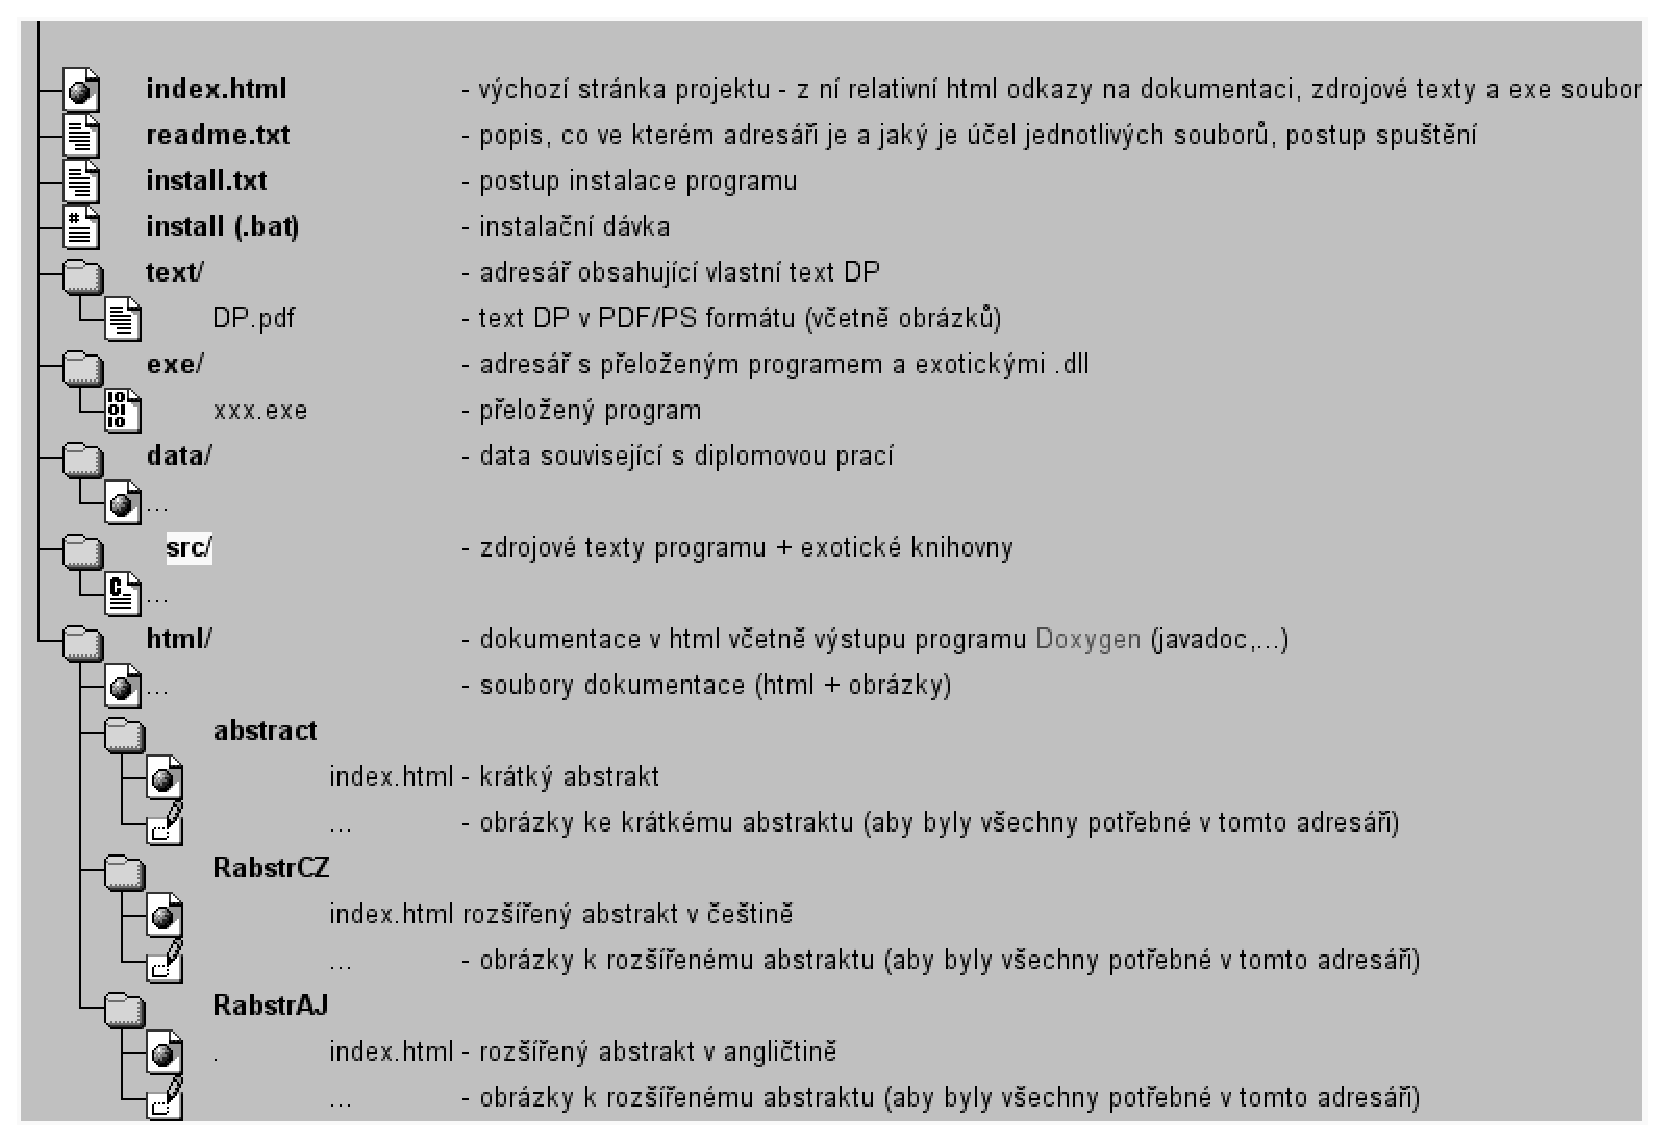
\includegraphics[width=14cm]{figures/seznamcd}
\caption{Seznam přiloženého CD --- příklad}
\label{fig:seznamcd}
\end{center}
\end{figure}

Na GNU/Linuxu si strukturu přiloženého CD můžete snadno vyrobit příkazem:\\ 
\verb|$ tree . >tree.txt|\\
Ve vzniklém souboru pak stačí pouze doplnit komentáře.

Z \textbf{README.TXT} (případne index.html apod.)  musí být rovněž zřejmé, jak programy instalovat, spouštět a jaké požadavky mají tyto programy na hardware.

Adresář \textbf{text}  musí obsahovat soubor s vlastním textem práce v PDF nebo PS formátu, který bude později použit pro prezentaci diplomové práce na WWW.

\end{document}
